%; whizzy document
% latex beamer presentation.
% platex, latex-beamer $B$G%3%s%Q%$%k$9$k$3$H$rA[Dj!%(B 

%     Tokyo Debian Meeting resources
%     Copyright (C) 2006 Junichi Uekawa

%     This program is free software; you can redistribute it and/or modify
%     it under the terms of the GNU General Public License as published by
%     the Free Software Foundation; either version 2 of the License, or
%     (at your option) any later version.

%     This program is distributed in the hope that it will be useful,
%     but WITHOUT ANY WARRANTY; without even the implied warranty of
%     MERCHANTABILITY or FITNESS FOR A PARTICULAR PURPOSE.  See the
%     GNU General Public License for more details.

%     You should have received a copy of the GNU General Public License
%     along with this program; if not, write to the Free Software
%     Foundation, Inc., 51 Franklin St, Fifth Floor, Boston, MA  02110-1301 USA

% $B<B9T=gHV(B
% sudo  ~/bin/usb-macbook-ir.c &
% real presentation (shell-command (concat "DISPLAY=:0.1 xpdf -fullscreen " (replace-regexp-in-string "tex$" "pdf"(buffer-file-name)) "&"))
% DISPLAY=:0.1 xpdf -fullscreen 

\documentclass[cjk,dvipdfm,14pt]{beamer}
% 14 seems like the max relevant value 
\usetheme{Warsaw}

%  preview (shell-command (concat "xpdf " (replace-regexp-in-string "tex$" "pdf"(buffer-file-name)) "&"))
%  presentation (shell-command (concat "xpdf -fullscreen " (replace-regexp-in-string "tex$" "pdf"(buffer-file-name)) "&"))


%http://www.naney.org/diki/dk/hyperref.html
%$BF|K\8l(BEUC$B7O4D6-$N;~(B
\AtBeginDvi{\special{pdf:tounicode EUC-UCS2}}
%$B%7%U%H(BJIS$B7O4D6-$N;~(B
%\AtBeginDvi{\special{pdf:tounicode 90ms-RKSJ-UCS2}}

\title{Binfmtc/realksh}
\subtitle{$B;qNA(B}
\author{$B>e@n(B $B=c0l(B dancer@debian.org}
\date{2006$BG/(B9$B7n(B28$BF|(B}
\logo{\includegraphics[width=8cm]{image200607/openlogo-light.eps}}

% $B;0BrLdBjMQ(B
\newcounter{santakucounter}
\newcommand{\santaku}[5]{%
\addtocounter{santakucounter}{1}
\frame{\frametitle{$BLdBj(B\arabic{santakucounter}. #1}
%$BLdBj(B\arabic{santakucounter}. #1
\begin{minipage}[t]{0.7\hsize}
 \begin{itemize}
 \item A #2\\
 \item B #3\\
 \item C #4\\
 \end{itemize}
\end{minipage}
}
\frame{\frametitle{$BLdBj(B\arabic{santakucounter}. #1}
%$BLdBj(B\arabic{santakucounter}. #1
\begin{minipage}[t]{0.7\hsize}
\begin{itemize}
\item A #2\\
\item B #3\\
\item C #4\\
\end{itemize}
\end{minipage}
\begin{minipage}[t]{0.2\hsize}
$BEz$($O(B:


\vspace{1cm}

{\huge \hspace{1cm}#5}
\end{minipage}}
}


\begin{document}
\frame{\titlepage{}}

\section{$B;~Be$NN.$l(B}

\begin{frame}
\frametitle{shell$B$H$O(B}
LL$B8@8l$N86;O7A(B
\end{frame}

\begin{frame}
\frametitle{shell$B$H$O(B}
\begin{minipage}[t]{0.3\hsize}
   \onslide<1->sh\\
   \onslide<2->\includegraphics[width=1\hsize]{image200609/bourne.png}
\end{minipage}
\begin{minipage}[t]{0.3\hsize}
   \onslide<1->csh\\
   \onslide<3->\includegraphics[width=1\hsize]{image200609/billjoy.png} 
\end{minipage}
\begin{minipage}[t]{0.3\hsize}
   \onslide<1->ksh\\
   \onslide<4->\includegraphics[width=1\hsize]{image200609/korn.png}
\end{minipage}
\end{frame}

\begin{frame}
\frametitle{shell$B$H$O(B}
\begin{itemize}[<+->]
 \item shell $B$O$J$s$@$+8@8l;EMM$,@)8B$5$l$F$$$F;H$$$K$/$$(B
 \item C $B$O$J$s$@$+5$7Z$K;H$($J$$$N$G(BLL$B$8$c$J$$(B
\end{itemize}
\end{frame}

\begin{frame}
\frametitle{C$B8@8l$N;~Be$NN.$l(B}
 \begin{itemize}[<+->]
  \item $B$b$7$+$7$F$"$^$j$O$d$C$F$$$J$$!)(B
  \item $B%+!<%M%k%3!<%G%#%s%0$J$II,MW$J>lLL$OB?$$(B
  \item emacs buffer $B$G(B eval $B$7$J$,$i%3!<%I$,$+$1$k8@8l$,$&$i$d$^$7$$(B
  \item $B$[$H$s$I$N%W%m%0%i%`8@8l$O%$%s%?%W%j%?E*$KF0:n$9$k%$%s%?%U%'!<%9(B
	$B$,$"$j!"%3%s%Q%$%k!&%j%s%/$N<j=g$r>JN,$G$-$k(B
  \item $B$[$H$s$I$N%W%m%0%i%`8@8l$K$OBPOC%$%s%?%U%'!<%9$,$"$j!"(B
	$B$?$a$7$J$,$i%3!<%I$,=q$1$k(B
 \end{itemize}
\end{frame}

\section{$B%D!<%k>R2p(B}
\subsection{binfmtc}

\begin{frame}
\begin{itemize}[<+->]
 \item C$B$r%9%/%j%W%H8@8l$_$?$$$K;H$$$?$$(B!
\end{itemize}
\end{frame}

\begin{frame}
\includegraphics[width=1\hsize]{image200609/binfmtc.eps}
\end{frame}

\begin{frame}
\begin{itemize}
 \item C$B$r%9%/%j%W%H8@8l$_$?$$$K;H$$$?$$(B!
\end{itemize}
\includegraphics[width=1.0\hsize]{image200609/upaccho.png}
\end{frame}


\subsection{realcsh}
\begin{frame}
\begin{itemize}[<+->]
 \item C$B$r%7%'%k$H$7$F;H$$$?$$!*(B
 \item csh$B$C$F$J$s$+0c$&$h$M!)(B
\end{itemize}
\end{frame}

\begin{frame}
\includegraphics[width=0.5\hsize]{image200609/realcsh.eps}
\end{frame}

\begin{frame}
\begin{itemize}
 \item C$B$r%7%'%k$H$7$F;H$$$?$$!*(B
 \item csh$B$C$F$J$s$+0c$&$h$M!)(B
\end{itemize}
\includegraphics[width=1.0\hsize]{image200609/realcsh-while.png}
\end{frame}

\subsection{realksh}
\begin{frame}
\includegraphics[width=0.5\hsize]{image200609/structure.eps}
\end{frame}

\begin{frame}
\begin{itemize}
 \item ksh $B$C$F$J$s$G(B kernel $B$8$c$J$$$s$@(B?
\end{itemize}
\includegraphics[width=0.8\hsize]{image200609/realksh-demo.png}
\end{frame}

\section{$B<B1i(B}
\begin{frame}
 
\end{frame}



\end{document}
